\documentclass[german,english,twoside,headsepline,titlepage=true]{scrartcl}
% Header, der in jedem meiner Dokumente drinhängt.
% Setzt Rechtschreibung, Hyperlinks, Schriftart und Typographie

\usepackage[]{babel}
\babeltags{de = german}

\usepackage{xparse}
\usepackage[colorlinks=true,linkcolor=blue,pdfborder={0 0 0}]{hyperref}
\usepackage{hyperxmp}
\usepackage{microtype}
%\usepackage[scale=3]{ccicons}


\usepackage[]{fontspec}
%\setmainfont[Fractions=On]{Linux Libertine O}
\setmainfont{Linux Libertine O}
\setsansfont{Linux Biolinum O}

\usepackage{todonotes}
\usepackage[left]{showlabels}
% Hier sollten meine wichtigsten Mathe Befehle zu finden sein.
% Weiter unten sind die spezielleren Befehle, die je nach dem
% vielleicht auskommentiert oder gelöscht werden sollten.

\usepackage{amssymb}
\usepackage[]{amsmath}
\usepackage{amsthm}
\usepackage{mathtools}

%tikz
\usepackage{tikz}
\usetikzlibrary{shadows}
\tikzset{node distance=3cm, auto}
\usepackage{pgfplots}

%Abkürzungen für Standardzahlmengen
\let\C\relax
\NewDocumentCommand\R{}{\mathbb{R}}
\NewDocumentCommand\Q{}{\mathbb{Q}}
\NewDocumentCommand\N{}{\mathbb{N}}
\NewDocumentCommand\C{}{\mathbb{C}}
\NewDocumentCommand\Z{}{\mathbb{Z}}
\NewDocumentCommand\A{}{\mathcal{A}}
\NewDocumentCommand\K{}{\mathbb{K}}
\NewDocumentCommand\p{}{\mathbb{P}}
\NewDocumentCommand\h{}{\mathbb{H}}
\NewDocumentCommand\F{}{\mathcal{F}}
\NewDocumentCommand\D{}{\mathcal{D}}
\NewDocumentCommand\lie{}{\mathcal{L}}
\NewDocumentCommand\jo{}{\mathfrak{J}}
\NewDocumentCommand\hol{}{\mathcal{O}}
\NewDocumentCommand\mer{}{\mathcal{M}}
\NewDocumentCommand\diff{}{\mathcal{E}}

% ein Paar Abbildungssachen.
\NewDocumentCommand\Supp{}{\operatorname{Supp}}
\NewDocumentCommand\id{}{\operatorname{id}}
\NewDocumentCommand\supp{}{\operatorname{supp}}
\NewDocumentCommand\rank{}{\operatorname{rank}}
\NewDocumentCommand\tr{}{\operatorname{tr}}
\NewDocumentCommand\ord{}{\operatorname{ord}}

%Pfeile und Stuff
\NewDocumentCommand\Ra{}{\Rightarrow}
\NewDocumentCommand\La{}{\Leftarrow}
\NewDocumentCommand\LRa{}{\Leftrightarrow}
\NewDocumentCommand\ra{}{\rightarrow}
\NewDocumentCommand\la{}{\leftarrow}

% Faktorräume
\NewDocumentCommand\quot{m m}{\left .\raisebox{.2em}{$#1$}\middle/\raisebox{-.2em}{$#2$}\right .}

% richtiges epsilon und phi
\let\epsilon\relax
\NewDocumentCommand\epsilon{}{\varepsilon}
\let\phi\relax
\NewDocumentCommand\phi{}{\varphi}

% Differential
\let\d\relax
\NewDocumentCommand\d{ O{} }{\operatorname{d}\hspace{-0.1em}#1}

%amsthm
%\theoremstyle{plain}
\theoremstyle{definition}
\newtheorem{thm}{Satz}[section]
\newtheorem{lemma}[thm]{Lemma}
\newtheorem{prop}[thm]{Proposition}
\newtheorem{cor}[thm]{Korollar}
%\theoremstyle{definition}
\newtheorem{defin}[thm]{Definition}
\newtheorem{bsp}[thm]{Beispiele}
%\theoremstyle{remark}
\newtheorem{rem}[thm]{Bemerkung}

% % Differentialgeometrie (Riemannsche Geometrie)
% \NewDocumentCommand\tang{ O{p} O{M}}{T_{#1}#2}
% \NewDocumentCommand\cotang{ O{p} O{M}}{T^\ast_{#1}#2}
% \NewDocumentCommand\del{ O{i} O{x} O{} }{\frac{\partial {#3}}{\partial {#2}^{#1}}}
% \NewDocumentCommand\delat{ O{p} O{i} O{x} O{} }{\left . \del[#2][#3][#4] \right |_{#1}}
% \NewDocumentCommand\christ{O{i} O{j} O{k} }{ \Gamma_{#1 #2}^{#3} }
% \NewDocumentCommand\g{m m}{\langle #1, #2 \rangle}
% \NewDocumentCommand\diam{}{\operatorname{diam}}
% \NewDocumentCommand\ric{}{\operatorname{ric}}
% \NewDocumentCommand\scal{}{\operatorname{scal}}
% \NewDocumentCommand\arsinh{}{\operatorname{arsinh}}

% % Bachelor-Arbeit
% \NewDocumentCommand\im{}{\operatorname{im}}
% \NewDocumentCommand\sm{}{\operatorname{sm}}
% \NewDocumentCommand\Reg{}{\operatorname{Reg}}
% \NewDocumentCommand\be{}{\mathfrak{B}}
% \NewDocumentCommand\pe{}{\mathfrak{P}}
% \NewDocumentCommand\res{}{\operatorname{res}}
% \let\S\relax
% \NewDocumentCommand\S{}{\mathcal{S}}
% \let\P\relax
% \NewDocumentCommand\P{}{\mathbb{P}}
% \NewDocumentCommand\Fix{}{\operatorname{Fix}}
% \NewDocumentCommand\Mat{}{\operatorname{Mat}}
% \NewDocumentCommand\SL{}{\operatorname{SL}}
% \NewDocumentCommand\GL{}{\operatorname{GL}}
% \NewDocumentCommand\PSL{}{\operatorname{PSL}}
% \let\Re\relax
% \NewDocumentCommand\Re{}{\operatorname{Re}}
% \let\Im\relax
% \NewDocumentCommand\Im{}{\operatorname{Im}}
% \NewDocumentCommand\Div{}{\operatorname{Div}}
% \NewDocumentCommand\Aut{}{\operatorname{Aut}}
% \NewDocumentCommand\Deck{}{\operatorname{Deck}}
% \NewDocumentCommand\runge{}{\mathfrak{h}}
% \NewDocumentCommand\fu{}{\mathfrak{U}}
% \NewDocumentCommand\dist{}{\mathcal{D}}

% Header, für sowas wie Bachelor- oder Master-Arbeiten.
% Folgende Parameter sind für documentclass vielleicht hilfreich:
% twoside: zweiseitiger Satz
% headsepline: Kopfzeile wird durch langen Strich getrennt
% titlepage = true: Es gibt eine Titel Seite und nicht nur ein Überschrift
% BCOR = 10mm: Binderandkorrektur einstellen

\usepackage{scrpage2}
\pagestyle{scrheadings}
% \ofoot{\pagemark}
% \lehead{Ich stehe in header\_artcl unter lehead}
% \rohead{\headmark}
\automark[subsection]{section}
%\automark*[subsection]{}

\usepackage[style=alphabetic,backend=biber]{biblatex}
\addbibresource{biblio.bib}

% \usepackage{makeidx}

% \NewDocumentCommand\init{m}{\emph{#1}\index{#1}}

% \makeindex

%%% Local Variables:
%%% mode: plain-tex
%%% TeX-master: "Bachelor"
%%% End:



\usepackage{chemformula}
\usepackage[exponent-product = \cdot]{siunitx}
\usepackage{graphicx}
\graphicspath{ {images/} }

% \usepackage{gnuplottex}
\newfontfamily\nfrac[Fractions=On]{Linux Libertine O}

\usepackage{pgfplots}

\addfontfeature{Fractions=On}



% Schmutztitel
\KOMAoption{twoside}{false}
\extratitle{
  ~
  \begin{center}
    \huge \textbf{Fakultät für Physik \& Astronomie}
  \end{center}
  ~
  \begin{center}
    \Large \textbf{Ruprecht-Karls-Universität Heidelberg}
  \end{center}
  \vfill
  \begin{center}
    \Large \textbf{Bachelor-Arbeit}\\[1ex]
    im Studiengang Physik\\
    vorgelegt von \\[1ex]
    \Large \textbf{Tim Adler}\\[1ex]
    geboren in Sinsheim
  \end{center}
  ~
  \begin{center}
    \huge \textbf{2016}
  \end{center}
}

\KOMAoption{twoside}{true}

\titlehead{Universität Heidelberg \\
  Fakultät für Physik \& Astronomie\\
  Im Neuenheimer Feld 226\\
  69120 Heidelberg}
\subject{Bachelor-Arbeit}
\title{Ein Konverter}
\author{Tim Adler}
\date{\today}
\publishers{Betreut durch Dr.\ Denis Pöhler und Prof.\ Dr.\ Ulrich Platt}
\uppertitleback{Tim Adler\\Eberlinweg 6\\69121
  Heidelberg\\tim \{at\} emrys-merlin.de}
\lowertitleback{
\textbf{Ein Konverter}\\
Bachelor-Arbeit im Fach Physik\\[\baselineskip]
Ruprecht-Karls-Universität Heidelberg\\
Fakultät für Physik \& Astronomie\\
Institut für Umweltphysik\\[\baselineskip]
\begin{tabular}[htbp]{l l}
Betreut durch & Dr.\ Denis Pöhler und Prof.\ Dr.\ Ulrich Platt\\
Beginn der Arbeit & some day \\
Datum der Abgabe & \today\\
\end{tabular}
\\[\baselineskip]
Diese Arbeit wurde mit Hilfe von {\LaTeX} und
  {\KOMAScript} gesetzt.}

\makeatletter
\hypersetup{
  pdftitle={\@title},
  pdfauthor={\@author},
  pdfdate={\@date}
}
\makeatother

\begin{document}

\pagenumbering{roman}
\selectlanguage{german}
\maketitle
\selectlanguage{english}

\listoftodos
\todo{ToDo-Liste entfernen.}
\newpage

\selectlanguage{german}

\subsubsection*{Zusammenfassung}
\label{sec:Zusammenfassung}

Ich mach was zu Konvertern
\todo{Zusammenfassung schreiben}

\selectlanguage{english}

\subsubsection*{Abstract}
\label{sec:abstract}

I try to build some sort of converter
\todo{Write abstract}

%%% Local Variables: 
%%% mode: latex
%%% TeX-master: "../Bachelor"
%%% End: 

\newpage

% Nur bis section, nicht bis subsection
\setcounter{tocdepth}{1}
\tableofcontents
\cleardoubleoddstandardpage{}
\pagenumbering{arabic}
Nothing to see yet
\cleardoubleoddstandardpage{}
\section{Theoretical background}
\label{sec:theory}

\subsection{Ozone chemistry and \ch{NO} to \ch{NO2} conversion}
\label{sec:chemistry}

This section lays the chemical groundwork for the construction of our
\ch{NO} to \ch{NO2} converter. First we will introduce the rate
coefficient to get a measure for the speed of a
reaction. Afterwards we will have a look at possible ways to generate
Ozone out of ambient air and then describe Ozone induced reactions
concerning Nitrogenoxides. This section is mainly inspired by and
taken from~\cite{bsc}.

\subsubsection{The rate coefficient}
\label{sec:rate}

During our conversion we will have many chemical reactions of the form

\begin{align*}
  \ch{A + B -> C + D}.
\end{align*}

Some of them will have positive, wanted effects, others describe side
effects and we want to suppress them as much as possible. However we
have only two parameters we can vary. The first is the Ozone
concentration, which we can vary slighty and very roughly and the
other one is the reaction pathlength and by that the reaction
time. Thus our best chance to select certain reactions is to set ther
reaction time to a value that corresponds to the different reaction
speeds of the equations, making sure that wanted reactions have enough
time to happen while simultaneously having the time too short for
unwanted reactions. Of cours this is only possible, if the wanted
reactions run faster than the unwanted ones. 

With this motivation in mind, we need a measure for the reaction
speed. Thinking of speed in this setting means to think of change of
compound concentration. In this section we will use $c$ to denote
concentrations. Using the above mentioned prototypic equation, we can
see that the change of concentration, i.\,e. $\dot c$, of the
different species are related by:
\begin{align*}
  -\dot c(A) = - \dot c(B) = \dot c(C) = \dot c(D).
\end{align*}

Lastly we want to get a connection of these derivatives to the educt
concentration. The probability for a reaction to take place should be
proportional both to $c(A)$ and $c(B)$ as the two particles need to
`meet'. Thus we expect
\begin{align}
  -\dot c(A) = - \dot c(B) = k \cdot c(A) \cdot c(B), \label{eq:rate}
\end{align}

where the proportionality constant $k$ ist called \emph{rate
  coefficient}. It is often given in units of
\si{\hertz\per\cubic\centi\meter}. This $k$ is our desired reaction
speed measure, as it describes concentration independently the
reaction time. 

In our case the Ozone concentration will often far exceed the
concentration of the other trace gases. This allows us to think of its
concentration as approximately constant. If we set $c(B)$ constant in
Equation~\eqref{eq:rate}, then we get a well known ordinary first
order differential equation with solution
\begin{align*}
  c(A,t) = c(A,0)\exp(kc(B)\cdot t).
\end{align*}

In this limiting case we see that the decay time is given by $\tau =
(kc(B))^{-1}$, such that the connection of $k$ to the reaction speed
becomes obvious.

\subsubsection{Ozone Generation}
\label{sec:theory-ozone}

In this section we will discuss the generation of Ozone (\ch{O3}) out of ambient
air. The main idea comes from the observation that stratospheric
\ch{O3} protects us from ultraviolet (UV) light. Thus Ozone needs to
have absorption bands there. Furthermore normally the Ozone layer is
not depleted, but regenerates itself, so there needs to be a reaction
cycle building Ozone out of ordinary Oxigen molecules (\ch{O2}).

The following equations describe the processes using UV photons to
generate and destroy Ozone. The cycle is ofthen referred to as
\emph{Chapman-Cycle}\todo{cite}. In some of the reactions an
additional molecule is necessary to assure momentum conservation. This
inert reaction participant is always denoted \ch{M}.

The first part of the cycle contains the reactions, that generate
\ch{O3} out of \ch{O2}

\begin{align}
  \ch{O2} + h\nu &\ch{-> 2 O(^3P)},\nonumber\\
  \ch{O(^3 P) + O2 + M} &\ch{-> O3 + M}. \label{eq:ozone}
\end{align}

We see that a photon splits an Oxygen molecule and the excited
Oxygen atom reacts with another \ch{O2} molecule to form Ozone. For
the first reaction to take place we need for the wavelength of the
photon $\lambda < \SI{242}{\nano\meter}$ to hold, i.\,e.\ we need a UV
photon. 

The next part of the cycle shows, how another UV photon can destroy
Ozone and create a ground state Oxygen atom. This Oxygen atom will
then be reexcited:

\begin{align}
  \ch{O3} + h\nu \ch{&-> O(^1 D) +
  O2}, \label{eq:split}\\
  \ch{O(^1 D) + M & -> O(^3 P) + M}.\nonumber
\end{align}

After this reaction there are two possible parts. Firt the $\ch{O}(^3
P)$ can reenter into Equation~\eqref{eq:ozone}, such that there is no
net change in Ozone or it could react to form \ch{O2} by the
following mechanisms

\begin{align*}
  \ch{2 O(^3 P) + M & -> O2 + M} \quad \text{and}\\
  \ch{O(^3 P) + O3 & -> 2 O2},
\end{align*}

leading to a net loss of Ozone. Introducing a UV light source with
wavelength less than \SI{242}{\nano\meter} will start the above
cycle. Since it contains sources and sinks for Ozone, we will reach an
equilibrium state with a limiting Ozone concentration. This
concentration will depend on multiple factors, which influence the
reaction speeds. First and foremost the intensity of the light source
at different wavelength segments determines if more Ozone is generated
than destroyed or not. An in depth analysis of this reaction system
has been carried out by\todo{cite}. For this work the main conclusion
is sufficient that using a Pen-Ray Hg-lamp within an alluminium coated
tube shifts the equilibrium in the above equations to a point where
there is enought Ozone generated for our purposes. The exact
characteristics of our generator were determined experimentally and
the results can be found in Section~\ref{sec:ozone}. 

\subsubsection{Ozone triggerd Nitrogenoxide reactions}
\label{sec:o-no}

In this section we will have a look at all reactions concerning
chemicals consisting of Nitrogen and Oxygen. Our aim is to convert
100\% of the Nitrogenmonoxide (\ch{NO}) to Nitrogendioxide
(\ch{NO2}). However introducing Ozone to the sample air can trigger
other reactions. If these lead to a net change of \ch{NO2} we have
additional effects to correct, if we want to determine the \ch{NO}
concentration. All reactions are given with their corresponding rate
coefficient $k$ which were taken from~\cite{bsc}. In
Section~\ref{sec:requirements} we will discuss the implications of the
reactions here on the setup of our converter.

The reaction we are mainly interested in and we want to be dominant is
the following

\begin{align*}
  \ch{NO + O3 & ->[$k=\SI{1.8e-14}{\hertz\per\cubic\centi\meter}$] NO2 + O2}.
\end{align*}

If this were the only reaction, we would have a one to one conversion
from \ch{NO} to \ch{NO2}. We would only have to make certain that
there is enough Ozone. However this is not the only reaction taking
place. Nitrogendioxide itself can be oxidized by Ozone to generate
Nitrogentrioxide (\ch{NO3}):

\begin{align*}
  \ch{NO2 + O3 ->[$k=\SI{3.5e-17}{\hertz\per\cubic\centi\meter}$] NO3 + O2}.
\end{align*}

Luckily, we see that the rate coefficients of the two reactions are
very different and the first ony is approximately three orders of
magnitude faster than the second one. Furthermore \ch{NO3} is again
not detectible by our measurement instrument. Also \ch{NO3} can react
again with \ch{NO2} to generate laughing gas

\begin{align}
  \ch{NO2 + NO3 + M
  <=>[$k=\SI{1.9e-12}{\hertz\per\cubic\centi\meter}$][$k=\SI{2.6e-11}{\hertz\per\cubic\centi\meter}$]
  N2O5 + M}. \label{eq:laughing}
\end{align}

As we can see the equilibrium of Equation~\eqref{eq:laughing} lies on the
side of the educts, so the effect should not be too large, if the
\ch{NO3} concentration can be kept low. In addition there is another
very fast reaction using \ch{NO3}

\begin{align}
  \ch{NO + NO3 ->[$k=\SI{6.9e-2}{\hertz\per\cubic\centi\meter}$] 2 NO2}.\label{eq:back}
\end{align}

Thus, if we keep the Nitrogentrioxide concentration low to begin with,
the above reaction implies that basically all of it should react with
\ch{NO} to form \ch{NO2}. Since \ch{NO3} is quickly destroyed by
photolysis, we can assume our measurement air to be \ch{NO3} free (at
least during day time measurements). Thus the molecules come either
from oxidizes \ch{NO2} or from twice oxidized \ch{NO}. In both cases
Equation~\eqref{eq:back} makes sure that our measurement is not distorted.


\subsection{Basics of fluid dynamics}
\label{sec:fluid}

One important aspect of this work consists in the understanding of the
different gas flows in the instrument. We need an estimate for the
mixing time of Ozone with the sample air and then we need to know how
long our mixing and reaction pathlength needs to be in order to
achieve a full conversion. These questions can all be answered using a
few basic principles from fluid dynamics. First we will have a look at
laminar flows in cylindric vessels (in our case tubes) to get a
connection between the flow and the maximum speed in the tube. Next we
have a look at diffusion of gases. As we only hav laminar flows,
diffusion is the only way mixing can take place, so we need an
estimate of the time this mixing takes. Lastly we will discuss
adsorption of some trace gases at teflon, silica gel and activated
carbon to better our understanding of the filtering effects in the
instrument. 

\subsubsection{Laminar flows in cylinders}
\label{sec:cylinder}

We are interested in what regime the gas transport in the tube
remains. Especially after the ozone enriched air is added to the
sample air, we would benefit from ab turbulent flow in the system as
it would acertain a faster mixing of the gases. To see whether we have
a laminar or a turbulent flow, we use the phenomenological \emph{Reynold's
number}

\begin{align*}
  \operatorname{Re} = \frac{\rho \cdot d \cdot \bar v}{\eta},
\end{align*}

where $\rho$ denotes the density of our gas, $d$ is a characteristc
length of the system, in our case the tube diameter, $\bar v$ is the
average velocity of the gas and $\eta$ its viscosity. As a rule of
thumb the flow in a cylinder will be laminar, if the Renold's number
is smaller than the critical Reynold's number
$\operatorname{Re}_{\text{c}} = 2300$ and the flow will be turbulent
if the number is higher than $3000$ (c.\,f.~\cite{maschbau}). In our
system we have $d = \SI{4}{\milli\meter}$, $\rho \approx
\SI{1.2}{\kilo\gram\per\cubic\meter}$ and $\eta \approx
\SI{17.1}{\micro\pascal\second}$. Furthermore we work with a flow of
$\Phi = \SI{2}{\liter\per\minute}$. With the above diameter this
leads to an average velocity of $\bar v =
\SI{2.7}{\meter\per\second}$. Using this data we compute the Reynold's
number to be

\begin{align*}
  \operatorname{Re} \approx 760 < 2300.
\end{align*}

Thus we see that we work solely in the laminar setting and we need to
understand the velocity distribution in this case in order to allow
enough time for mixing and the chemical reactions to take place. The
law behind the flow in a cylindric tube is called
\emph{Hagen-Poiseulle} and we follow the exposition used
in~\cite{gerthsen} to derive it.

Denote by $r_0$ the inner radius of our tube and by $l$ its length. We
assume that we are in the equilibrium state, such that all forces need
to add to zero. We look at a cylinder with radius $0 \leq r \leq
r_0$. To have a nonzero flow, we need a pressure difference at the two
ends of the tube dentode $\Delta p$. The force exerted on the cylinder
by the pressure is given by
\begin{align*}
  F_b = - \pi r^2 \Delta p,
\end{align*}

where the minus sign is introduced because the force points in the
opposite direction of the pressurre gradient. On the boundary of our
cylinder we have friction. The force exerted by 
it is proportional to the area of friction, i.\,e.\ the cylinder
barrel and to difference in velocity between the fluid within the
cylinder and without, since we have to look at an infinitesimal anulus
around the boundary, we get a proportionality to the velocity gradient
$\frac{\d[v]}{\d[r]}$. Thus the force of friction takes the form

\begin{align*}
  F_f = \eta \cdot 2\pi r \cdot l \cdot \frac{\d[v]}{\d[r]}.
\end{align*}

We are at an equilibrium state, thus we need $F_b = F_f$ for all
possible $r$ to hold. This leads us to the following differential
equatio for the velocity

\begin{align*}
  \frac{\d[v]}{\d[r]} = - \frac{\Delta p}{2l\eta} r
\end{align*}
 
whic can be directly integrated. Using the boundary condition $v(r_0)
= 0$, i.\,e.\ the fluid sticks at the wall of the tube, we yield

\begin{align}
  v(r) = v_0 \left ( 1 - \left( \frac{r}{r_0} \right)^2 \right) \quad
  \text{with }\ v_0 \coloneqq \frac{\Delta p r_0^2}{4 l \eta}. \label{eq:v}
\end{align}

This can be further integrated to yield the flow $\Phi$ of the system

\begin{align*}
  \Phi = \int_A v(r) \d[A] = 2\pi \int_0^{r_0} v(r)r \d[r] = \frac{\pi
  r_0^4}{8\eta l} \cdot \Delta p.
\end{align*}

This is the standard form of the Hagen-Poiseulle law. One remarkabel
obersvation is that there is a power four law between the radius of
the tube and the flow. More interesting for us is the relation between
the average velocity $\bar v$ and the maximum velocity $v_0$ at the
center of the pipe

\begin{align*}
  \bar v = \frac{\Phi}{\pi r_0^2} = \frac{\Delta p r_0^2}{8\eta l} \stackrel{\eqref{eq:v}}{=} \frac{v_0}{2}.
\end{align*}

So we see that at the center the the velocity is twice as large as the
average. We need to keep this effect in mind when it comes to compute
the dwell time of our gases.

\subsubsection{Diffusion}
\label{sec:diffusion}

As was shown in the previous section, the gas flows laminarly through
our instrument. Thus the only mechanism by which gas mixing can occur
is \emph{diffusion}. Therefore we we want an estimate for the time it
takes for diffusion to take place. This exposition drew inspiration
from~\cite{fluid}.

We are interested in the evolution of the concentration $n$ of a
species. Fick's first law states that the flow $\Phi$ of the species
is proprotional to the concentration gradient $\nabla n$ and that the
species flows from higher to lower concentration. We yield

\begin{align*}
  \Phi = - D \nabla n,
\end{align*}
where $D > 0$ is called the \emph{diffusion constant}. Assuming no
sources and sinks and using the continuity equation for fluids, we
arrive at Fick's second law

\begin{align*}
  \dot n = - \nabla \Phi = \nabla (D \nabla n) = D \cdot \Delta n,
\end{align*}
where for the last equation we assumed and istotrope medium, i.\,e.\
$\nabla D = 0$. This is a second order linear partial differential
equation and for arbitrary boundary conditions it can become
arbitrarily hard to solve. Since we are mostly interested in the
diffusion of species at small time scales, we can assume our vessel
inifinitely large. With this the equation becomes accessible via
Fourieranalysis. Let

\begin{align*}
  \hat n(k,t) = \mathcal{F}[n](k,t)
\end{align*}
be the fouriertransform of $n$ with regard to the three spatial
coordinates $x$. Using the known relation $\mathcal{F}[\partial_{x_j}
n](k,t) = -ik_j \hat n(k,t)$, we can transform the equation to

\begin{align*}
  \partial_t \hat n(k,t) =  - Dk^2 \hat n(k,t)
\end{align*}

an linar first order ordinary differential equation, with the well
known solution

\begin{align}
  \hat n(k,t) = c(k) \cdot \exp(-Dk^2 t). \label{eq:sol-ft}
\end{align}

To determine $c(k)$, we need to introduce an initial value. We again
work with an idealistic model. We will later on be interested in the
diffusion of one molecule. Therefore we work with the initial
condition
\begin{align*}
  n(x,0) = n_0 \delta(x),
\end{align*}
i.\,e.\ all the species (or for $n_0 = 1$: the particle) is localized
at one point for $t = 0$. We can fourietransform this initial
condition, too, and yield

\begin{align*}
  \hat n(k,0) = n_0.
\end{align*}
Plugging this into Equation~\eqref{eq:sol-ft}, we get

\begin{align*}
  \hat n(k,t) = n_0 \exp(-Dt \cdot k^2).
\end{align*}
This is a Gaußian function with regard to the variable $k$. If we want
the solution in terms of $x$ we need the inverse Fourier transform of
$\hat n$. However, we know that the Gauß function is an Eigenfunction
of the Fouriertransform (and its invers). Additionally the total
concentration needs to be the same for all times $t$. Thus we yield

\begin{align*}
  n(x,t) = \frac{n_0}{(2\pi \cdot 2Dt)^{3/2}} \cdot \exp \left(
  -\frac{1}{2} \cdot \frac{x^2}{2Dt} \right).
\end{align*}
We have found the solution to Fick's second law. This allows us to
describe the statistic behaviour of a particle undergoing
diffusion. Setting $n_0 = 1$, we arrive at the probability
distribution for the particle, which is just a Gaußian distribution
with a timedependent variance. We see that the expectation value of
the position $\langle x \rangle$ is always 0. However the standard
deviation $\sigma = \sqrt{2Dt}$
grows larger over time, such that vor the \emph{mean squared
  displacement}, we yield the following relation

\begin{align}
  \langle x^2 \rangle = \sum_{j=1}^3 \langle
  x_j^2 \rangle = \sum_{j=1}^3 \sigma^2 = 3 \cdot 2Dt, \label{eq:mqd}
\end{align}

where we used $\langle x \rangle = 0$. This mean squared displacement
can now be used as a measure to gauge the distance travelled by a
molecule. We will apply it to gauge the time needed for a new gas
species (in our case Ozone) to fill a volume sufficiently for the
chemical reactions to take place.

\subsubsection{Adsorption}
\label{sec:adsorption}
\todo{find something out and write something about diffusion}

\subsection{Technical requirements for the converter}
\label{sec:requirements}

The above considerations lead to some technical requirements in the
construction of our converter. First and obviously we need to use well
filtered air in the Ozone generator as not to introduce other trace
gases which would disturb the measurement. The normal procedure
consists of using an activated charcoal, a silica gel and a particle
filter. However, one problem is that \ch{NO} is hardly soluble in
water and thus passes all these filter barriers. After the Ozone
generation it will react with it and lead to an additional \ch{NO2}
signal, which cannot be neglected. To remove it, one can add
another silica gel filter after the generator. \ch{NO2} is well
adsorbed within, which should lead to the desired reduction of the
error. However, Ozone is also adsorbed in Silica. Luckily, the
adsorption capacity for Ozone is much worse than for Nitrogen
Dioxide. So we would expect the filter to be quickly saturated by
Ozone, so that it can pass, while still blocking \ch{NO2}. To make
this work, we also have to add some extra pathlength after the
generator to make sure that the oxidization takes place before the gas
passes the Silica gel filter.

The next restriction is that we need a nigh \SI{100}{\%} conversion of
\ch{NO} to \ch{NO2}. This leads to three considerations. Firstly, we
need enough time for the mixing of the ozone with the sample air to
take place. Secondly, we need enough time for the actual reaction to
take place. Thirdly, we need the time to be short enough, such that we
do not loose to much \ch{NO2} to further oxidation.

Concering our first consideration, we have to look at
Section~\ref{sec:fluid} to estimate the mixing time. As we work with
laminar flows in the reaction path (c.\,f.\ Sec.~\ref{sec:cylinder}),
the mixing will be dominated by diffusion. Thus we use the mean
squared displacement to estimate the time the Ozone takes to cross the
tube diameter. In our case we use tubes with $d =
\SI{4}{\milli\meter}$ and the diffusion constant for Ozone in air was
taken to be $D = \SI{0.137}{\square\centi\meter\per\second}$ (at $T =
\SI{298}{\kelvin}$ and $p = \SI{1}{\text{bar}}$
c.\,f.~\cite{diff-ozone}). With these values we get
\begin{align*}
  t_{\text{mix}} = \frac{d^2}{6\cdot D} = \SI{0.195}{\second}
\end{align*}

Turning towards considerations two and three, we need to gauge the
reaction times. For this we have to set a desired conversion
ratio. For our estimates work with a ratio of \SI{99}{\%}. 
Since the Ozone generator will supply an
overabundance of \ch{O3}, we can use the linear ordinary
differential equation approximation introduced in
Section~\ref{sec:rate}. Thus the conversion ratio is
given by
\begin{align*}
  \exp(-kc(\ch{O3})\cdot t),
\end{align*}
where $t$ is the reaction time. $1$ stands for no
conversion at all (i.\,e.\ no decrease in the educt concentration) and
$0$ stands for complete conversion. For \SI{99}{\%} we need
\begin{align}
  kc(\ch{O3}) \cdot t_{\text{react}} \gtrsim 4.6. \label{eq:react-bound}
\end{align}
As a lower bound for the Ozone concentration we use
\begin{align*}
  c(\ch{O3}) = \SI{2}{ppm} = \SI{4.996e13}{\per\cubic\centi\meter} 
\end{align*}
and using $k = \SI{1.8e-14}{\hertz\per\cubic\centi\meter}$, we yield
the following natural time scale
\begin{align*}
  \tau^{-1} & = k c(\ch{O3}) = \SI{0.90}{\hertz}.
\end{align*}

Together with Equation~\eqref{eq:react-bound} this leads to

\begin{align*}
  t_{\text{react}} \gtrsim \SI{5.1}{\second}.
\end{align*}

Using $t_{\text{react}}$ to compute the conversion ratio of
$\ch{NO2}$ to $\ch{NO3}$, we get \SI{0.9}{\%}. So with this reaction
time we should expect about a \SI{2}{\%} error in the retrieved
\ch{NO} concentration. Hopefully, the results will be better than
that, as some of the produced \ch{NO3} will (as described in
Section~\ref{sec:o-no}) quickly degrade to \ch{NO2} and the Ozone
concentration is likely to be underestimated.

As a last step we want to translate the needed mixing and reaction
time
\begin{align*}
  t = t_{\text{mix}} + t_{\text{react}} = \SI{5.3}{\second}
\end{align*}
to be converted to its associated pathlength. Using the applied flow
of $\Phi = \SI{2}{\liter\per\minute}$, we can compute the average
speed of the gas to be
\begin{align*}
  \bar v = \frac{\Phi}{\pi r^2} = \SI{2.7}{\meter\per\second}. 
\end{align*}
As was described in Section~\ref{sec:cylinder} this corresponds to a
maximal speed in the center of the tube of

\begin{align*}
  v_0 = 2\cdot \bar v = \SI{5.4}{\meter\per\second}.
\end{align*}

Using these two speeds we get

\begin{align*}
  \bar l & = \SI{14.31}{\meter} \quad \text{and}\\
  l_0 & = \SI{28.62}{\meter}
\end{align*}
as our pathlengths.

For the experiment we oriented at $\bar l$, as the maximum speed is
only relevant for a rather small cross section of the
cylinder. Most experiments were performed at $l = \SI{10}{\meter}$
accepting a slightly worse \ch{NO} conversion ratio at the upside of a
smaller loss to \ch{NO3}. As all these estimates were intended as a
worst case, we expect even a \SI{10}{\meter} reaction path to be
sufficient for acceptable results.

\subsection{The physics behind CE-DOAS}
\label{sec:ce-doas-physics}

In the following sections we will discuss the physical concepts
necessary to understand the Cavity Enhance Diffirential Absorption
Spectroscopy (CE-DOAS). First, we will investigate the Lambert-Beer
Law. This leads directly to the so called \emph{Longpath}-DOAS
instrument. As the name already indicates, those need a long
lightpath, since normally the absorption crosssections are very
small. Thus lastly we introduce the \emph{cavity enhancement} to
overcome this restriction.

The presentation follows mostly~\cite{fp58} with a few inspirations
taken from~\cite{bsc} and~\cite{platt2008differential}.

\subsubsection{The Lambert-Beer Law}
\label{sec:lambert-beer}

The \emph{Labert-Beer Law} ist the underlying principle behind the
main measurement method used in this work. It concerns itself with the
evolution of the light intensity $I_0$ which propagates a certain
distance $L$ through air. It assumes an exponential decay over $L$, so
we can write

\begin{align}
  I(\lambda, L) = I_0(\lambda) \cdot \exp[-\epsilon(\lambda) \cdot
  L], \label{eq:lb-easy}
\end{align}

where $\epsilon$ is called \emph{absorption coefficient}. This
coefficient contains all the influences of the matter on the
absorption and can thus be split to account for the different
absorption and scattering mechanisms:

\begin{align*}
  \epsilon = \epsilon_a + \epsilon_R + \epsilon_M,
\end{align*}

where $\epsilon_a$ denotes the absorption and scattering due to the
trace gases, $\epsilon_R$ denotes Rayleigh scattering and $\epsilon_M$
Mie scattering. Next we want to understand the influence of the trace
gases on $\epsilon_a$ a little better. The absorption should be
proportional to the concentration of the gases, so we write

\begin{align}
  \epsilon_a(\lambda) = \sum_{i=1}^n \sigma_i(\lambda) \cdot \bar c_i, \label{eq:lb-abs}
\end{align}

where $i$ sums over all the trace gases present in the penetrated
air, $\bar c_i$ is the associated average concentration and $\sigma_i$
is calld \emph{absorption crosssection}. For the above formula to be
useful to determine the concentration of our trace gases, we need to
have a very homogenous air sample, so that we can assume that the
concentration within it is constant. As we will see this assumption is
sensible vor CE-DOAS, if one works with Longpath-DOAS measurements one
has to work with other parameters, e.\,g.\ the collon density.

Equations~\eqref{eq:lb-easy} and~\eqref{eq:lb-abs} now contain the central idea for our
spectroscopic method. We can measure the intensity spectra $I$ and
$I_0$, we can also determine the pathlength $L$. If we now want to
compute the concentration of our trace gases, we only need the
absorption crosssections, which can be found in the
literature.\todo{cite} Thus lastly we introduce the \emph{Optical
  Density} 

\begin{align*}
  D(\lambda) = \ln \left(\frac{I(\lambda)}{I_0(\lambda)}\right) = - L
  \cdot \sum_{i=1}^n \sigma_i(\lambda) c_i,
\end{align*}

which contains all the necessary information.

\subsubsection{The DOAS method}
\label{sec:doas}

Differential Optical Absorption Spectroscopy uses the Lambert-Beer Law
to compute the concentrations of trace gases in the air. There are a
few more technicalities we need to respect. First of all, we must have
a look at the absorption crosssections of different trace gases. If we
want to be able to discern different gases and even compute their
concentration, we need the crosssections to be sufficiently
different.

As can be seen in Figure\todo{include picture of crosssection}  the
crosssections can be separated into two parts: 

\begin{align*}
  \sigma = \sigma^b + \sigma'.
\end{align*}

One ($\sigma^b$) only weakly
wavelength dependent and similar for all gases and a narrowband
structure ($\sigma'$) on top which differs strongly for different species. This
narrowband structure is what will allow us to discern the gases. It is
called the \emph{differential band}. Hence the name of the
method. Putting what we used so far into the Lambert-Beer equation we
yield

\begin{align*}
  I(\lambda, L) & = I_0(\lambda) \exp \left ( \sum_{i=1}^n L \cdot
                  (\sigma^b_j(\lambda) + \sigma'_j(\lambda))\cdot c_j + L[\epsilon_R +
                  \epsilon_M]\right) \\
                & = I'_0(\lambda) \exp \left( \sum_{i=1}^n L \cdot
                  \sigma'_j(\lambda) \cdot c_j \right),
\end{align*}

where we collected all the broadband structure within $I'_0$. This
makes sense, as our $I_0$ spectrum will never be free of the Rayleigh
and Mie scattering processes and thus are already taken into
account. Furthermore can residual broadband structure be handled in
the fitting process by adding a polynomial function. Thus we fit

\begin{align}
  f(\lambda) = - \sum_{i=1}^n c_i \cdot L \cdot \sigma'_i(\lambda) +
  \sum_k a_k \lambda^k \label{eq:doas-fit}
\end{align}

to the Optical Density, where the concentrations $c_i$ and the polynomial
coefficients $a_k$ are to be determined. 

One other technical aspect we have to keep in mind, is how to get the
absorption crosssections. They have been determined by various
methods. Some have been computed theoretically other have been
measured with a very high resolution. So we are given the
crosssections, however, we need to adapt them to the spectrometer used
in our measurement instrument, since it has a far lower
resolution. The effect of this lower resolution is that narrow
emission lines are smeared out. This smearing out is called
\emph{instrument function}. To determine it, we can measure the
spectrum of an \ch{Hg}-lamp and use one of the
(normally very narrow) emission lines as a convolution kernel. The
narrow line is broadened and we can assume that all other used
measurements are broadened by the same amount. So if we convolute our
crosssections with this measured \ch{Hg}-line, we will compensate for
the lower resolution. This step has to be done before the actual fit
and in Equation~\eqref{eq:doas-fit} the convoluted crosssections have
to be used.

This plain DOAS method is used as measurement method on
Section~\ref{sec:ozone-setup}. 

\subsubsection{The CE-DOAS method}
\label{sec:ce-doas}

Since the absorption coefficents $\epsilon$ are so small, we need a
very long pathlength $L$ to see a signal in the DOAS method. One
possibility is to really use a very long geometrical pathlength using
mirrors and telescopes. With this we are able to obtain pathlengths
between \num{1} and \SI{10}{\kilo\meter}\todo{cite}. These so called
\emph{Longpath-DOAS} instruments have advantages, but also a few
disadvantages one of them clearly being that we need a lot of space
and in the process we average the concentration of our trace gases
over a large area.

An alternative approach is to increase the lightpath by the use of
optical instruments, i.\,e.\ mirrors. Using two highly reflective
mirrors we can obtain very large optical pathlengths, while still
having a managable geometrical pathlength. The price we pay by taking
this approach lies in the fact that now our pathlength becomes
wavelength dependent as this is true for the reflectivity of all
highly reflecting mirrors. 

In this paragraph we will generalize the DOAS approach keeping in mind
that our pathlength is not constant anymore. On the way we try to
separate two effects on the pathlength. First the shortening due to
the absorption by the trace gases and secondly the influence by the
reflectivity.

The CE-DOAS method was used for the measurements in
Sections~\ref{sec:silica} to~\ref{sec:vehicle}. 

The geometrical setup is the following:\todo{setup}

where we have two mirrors with reflectivity $R_i$, transmittance $T_i$
and absorption $A_i$. We have

\begin{align*}
  R_i + T_i + A_i = 1 \quad i \in{1,2}.
\end{align*}

Furthermore we have the transmittance $T_g$ of the gas in the
cavity. For this we get from the Lamert-Beer law

\begin{align*}
  T_g = \exp(-\epsilon d),
\end{align*}

where $d$ is the length of our cavity. If we take some intensity
$I_{\text{in}}$ entering the cavity and we want to compute the outgoing
intesity $I_{\text{out}}$ we get a geometric series

\begin{align*}
  I_{\text{out}} & = I_{\text{in}} T_1 T_2 T_g \sum_{n=0}^\infty R_1^n R_2^n T_g^{2n}\\
  & = I_{\text{in}} T_1 T_2 T_g \cdot \frac{1}{1 - R_1R_2T_g^2},
\end{align*}

where for the last equation we need $R_1R_2T_g^2 < 1$ to hold, which
is clearly true since all entering variables lie between 0 and 1.

With this formula we are able to compute the sample air intensity $I$
as well as the zero air (i.\,e.\ the trace gas free) intensity $I_0$
depending on the different reflectivities and transmittances. To do
this we will use a few approximations, which are listed in the
following

\begin{enumerate}
\item $I_{\text{in}}$ is the same for both $I$ and $I_0$. This means
  we are neglecting any fluctuations in the light source intensity
  coming from temperature instabilities or other optomechanic effects.
\item We assume $R_1 \approx R_2 \eqqcolon R \approx 1$, meaning $(R -
  1) \ll 1$. Since we use hihgly reflective mirrors this assumption
  seems reasonable.
\item We assume $\epsilon \cdot d \ll 1$ for both sample and zero
  air. Furthermore we assume the transmittances for both zero air and
  sample air to be equal to first order. We write $T_g \approx
  T_{g,0}$. This seems also reasonable as the absorption in air is
  comparativly weak and our geometrical pathlength is in the order of
  magnitude of \SI{1}{\meter}.
\item We assume  $(R - 1) + \epsilon d \ll 1$, too. This is only a
  slightly stronger condition then the above mentioned two, but
  necessary. 
\item We assume to be allowed to neglect higher order monomials of the
  form $(R-1)^i(\epsilon d)^j$  with $i+j \geq 2$, $i,j \in \N_0$.
\end{enumerate}

In the following we will always refer to the number of the above
mentioned assumptions, when used. The approximations carried out below
are described in~\cite{platt2009} and~\cite{fiedel2003}.

The information of our trace gas concentration should in this setup
still be obained by comparing $I$ and $I_0$. We still expect an
exponential factor between the two so we introduce the \emph{Cavity
  Enhanced Optical Density} $D_{\text{CE}}$ by

\begin{align}
  I(\lambda) = I_0(\lambda) \cdot \exp(- D_{\text{CE}}) = I_0(\lambda)
  \cdot \exp(-\delta(\lambda) \cdot L_{\text{eff}}(\lambda)),
\end{align}

where $\delta \coloneqq \epsilon - \epsilon_0$ is the difference
between the absorption coefficients of sample and zero air, i.\,e.\ the
absorption coefficient of the trace gases and $L_{\text{eff}}$ is the
wavelength dependent \emph{effective pathlength} of the system. Next
we will take a closer look at $D_{\text{CE}}$.

\begin{align}
  D_{\text{CE}}(\lambda) & \coloneqq \ln\left(
                           \frac{I_0(\lambda)}{I(\lambda)}\right)\nonumber\\
                         & = \ln\left ( \frac{I_{\text{in}}T_1T_2T_{g,0}(1 -
                           (RT_{g,0})^2)^{-1}}{I_{\text{in}}T_1T_2T_g(1 -
                           (RT_g)^2)^{-1}}\right)\nonumber\\
                         & \stackrel{3.}{\approx} \ln\left( \frac{1 -
                           (RT_g)^2}{1 - (RT_{g,0})^2}\right)\label{eq:d_ce},
\end{align}

where the wavelenght dependencies were dropped after the first
equation to preserve clarity. 

To evaluate this expression further we
first have a look at the separate expression $(RT)^2$:

\begin{align}
  [RT]^2 & = [R \exp(-\epsilon d)]^2 \nonumber\\
         & \stackrel{3.}{\approx} [R \cdot(1 - \epsilon d)]^2 \nonumber\\
         & = [(1 + (R - 1))\cdot (1 - \epsilon d)]^2 \nonumber\\
         & \stackrel{5.}{\approx} [1 - (1 - R + \epsilon d)]^2 \nonumber\\
         & \stackrel{4.}{\approx} 1 - 2 \cdot (1 - R + \epsilon d)\label{eq:rt}.
\end{align}

Inserting Equation~\eqref{eq:rt} into Equation~\eqref{eq:d_ce} we
yield

\begin{align}
  D_{\text{CE}} & \approx \ln \left ( \frac{1 - (1 - 2\cdot ( 1- R +
  \epsilon d))}{1 - (1 - 2 \cdot (1 - R + \epsilon_0 d))}\right)\\
  & = \ln \left ( \frac{1 - R + \epsilon d}{1 - R + \epsilon_0
    d}\right) \\
  & = \ln \left ( 1 + \frac{ \delta d}{1 - R + \epsilon_0 d}\right) \quad
    \text{with } \delta \coloneqq \epsilon - \epsilon_0.
\end{align}

This last equation can be reformulated to

\begin{align}
  \exp(D_{\text{CE}}(\lambda)) - 1 = \frac{I_0(\lambda)}{I(\lambda)} -
  1 = \frac{d}{1 - R(\lambda) + \epsilon_0(\lambda) d} \cdot
  \delta(\lambda)\label{eq:i-1}, 
\end{align}

where all the trace gas information is bundled in $\delta(\lambda)$
and the other right hand side parts are trace gas independent.

In a next step we want anlogously $D_{\text{CE}}$ to be given by a
pathlength multiplied by $\delta$. Thus we define

\begin{align}
  L_{\text{eff}}(\lambda) \coloneqq \frac{D_{\text{CE}}(\lambda)}{\delta(\lambda)}.
\end{align}

In this equation we can enter Equation~\ref{eq:i-1} solved for
$\delta$ and get

\begin{align}
  L_{\text{eff}} = \frac{D_{\text{CE}}}{\exp(D_{\text{CE}}) - 1} \cdot
  \underbrace{\frac{d}{1 - R + d\epsilon_0}}_{\eqqcolon L_0}.
\end{align}

We see that with this definition of $L_0$ it is completely independent
of any trace gas influence and hence all the trace gas dependence is
restricted to the first term. Furthermore we see that $L_0$ directly
depends on the mirror reflectivity. All in all $L_0$ depends only on
the geometry of our setup (if we assume $\epsilon_0$ to be fixed) and
we have reached the desired separation of $L_{\text{eff}}$.

Looking only at the definition of $L_0$ and comparing it to
Equation~\eqref{eq:i-1}, we yield

\begin{align}
  \delta \cdot L_0 = \frac{I_0}{I} - 1 \eqqcolon D_{\text{eff}}, \label{eq:ce-central}
\end{align}

where $D_{\text{eff}}$ is calle \emph{Effective Optical Density}.This
is the central equation for the CE-DOAS evaluation. $I$ and $I_0$ are
measured $L_0$ only depends on the geometry, so the only place, where
the trace gas concentrations enter are through $\delta$, which makes
it very easy for us to fit the concentrations.

In addition this equation also allows us to determine the pathlength
$L_0$. Using Helium as sample air we have a rather large difference
and well known $\delta$, which we can then use to fit
$L_0$.

In the actual evaluation we then take, as in the DOAS evaluation, the fit function

\begin{align*}
  f(\lambda) \coloneqq L_0(\lambda)\cdot\sum_{j=1}^n \sigma_j(\lambda)
  \cdot c_j + \sum_i a_i \lambda^i,
\end{align*}

where the parameters $c_j$ and $a_i$ are fitted to
$D_{\text{eff}}$. This is done using the leas square methods. The
polynomial is again added to compensate for broadband structure.

%%% Local Variables: 
%%% mode: latex
%%% TeX-master: "../Bachelor"
%%% End: 

\cleardoubleoddstandardpage{}
\subsection{Startup behaviour of the ozone generator}
\label{sec:ozone}

During these first experiments, I wanted to assure that the ozone
generator produces enough ozone. More precisely I was interested,
whether the ozone could penetrate the Silica gel and how long it would
take for it to succeed. In a last step I wanted to calibrate the relation
between the ozone production and the applied electrical current at the
mercury lamp.

\subsubsection{Setup}
\label{sec:ozone-setup}

The following experiments were all conducted using the setup described
in Section~\ref{sec:ozone-setup}. Since the cuvette had to be entered
in and removed from the lightpath manually, the time resolution had to
be reduced to \SI{5}{\minute}. In a first step I measured the startup
\ch{O3} transmission through the silica gel filter after a one week
stop of the generator. Secondly, I researched the startup time
necessary after shorter stops. Lastly, I noted the influence of the
lamp current on the ozone concentration. Using this setup it was
impossible to measure the generator's \ch{NO2} productoin. Since the
concentration should be around the \ch{NO_x} concentration in ambient
lab air, it should be no more than a few \si{ppb}. This is far below
the detection limit of a `longpath' DOAS instrument with a pathlength
of \SI{8.6}{\centi\meter} and a LED peak at $\lambda \approx
\SI{290}{\nano\meter}$.

\subsubsection{Results}
\label{sec:ozone-results}

As a zeroth, qualitative experiment I turned on the generator
and succeeded in perceiving an ozone signal. After that I shut down the generator
for one week. The startup behaviour afterwards can be seen in
Figuer~\ref{fig:long-stop}. It shows that the generator takes about
\SI{35}{\minute} before it reaches its stable plateau of around
\SI{250}{ppb} ozone. During this experiment the flow was constantly
set to $\Phi_{\ch{O_3}} = \SI{0.03}{\liter\per\minute}$. It stands to
argue that the startup time could be shortened by increasing the flow,
however, as shall be seen shortly, if the
generator is used regularly, this procedure seems unnecessary.

\begin{figure}[htbp]
  \centering
  % GNUPLOT: LaTeX picture with Postscript
\begingroup
  \makeatletter
  \providecommand\color[2][]{%
    \GenericError{(gnuplot) \space\space\space\@spaces}{%
      Package color not loaded in conjunction with
      terminal option `colourtext'%
    }{See the gnuplot documentation for explanation.%
    }{Either use 'blacktext' in gnuplot or load the package
      color.sty in LaTeX.}%
    \renewcommand\color[2][]{}%
  }%
  \providecommand\includegraphics[2][]{%
    \GenericError{(gnuplot) \space\space\space\@spaces}{%
      Package graphicx or graphics not loaded%
    }{See the gnuplot documentation for explanation.%
    }{The gnuplot epslatex terminal needs graphicx.sty or graphics.sty.}%
    \renewcommand\includegraphics[2][]{}%
  }%
  \providecommand\rotatebox[2]{#2}%
  \@ifundefined{ifGPcolor}{%
    \newif\ifGPcolor
    \GPcolorfalse
  }{}%
  \@ifundefined{ifGPblacktext}{%
    \newif\ifGPblacktext
    \GPblacktexttrue
  }{}%
  % define a \g@addto@macro without @ in the name:
  \let\gplgaddtomacro\g@addto@macro
  % define empty templates for all commands taking text:
  \gdef\gplbacktext{}%
  \gdef\gplfronttext{}%
  \makeatother
  \ifGPblacktext
    % no textcolor at all
    \def\colorrgb#1{}%
    \def\colorgray#1{}%
  \else
    % gray or color?
    \ifGPcolor
      \def\colorrgb#1{\color[rgb]{#1}}%
      \def\colorgray#1{\color[gray]{#1}}%
      \expandafter\def\csname LTw\endcsname{\color{white}}%
      \expandafter\def\csname LTb\endcsname{\color{black}}%
      \expandafter\def\csname LTa\endcsname{\color{black}}%
      \expandafter\def\csname LT0\endcsname{\color[rgb]{1,0,0}}%
      \expandafter\def\csname LT1\endcsname{\color[rgb]{0,1,0}}%
      \expandafter\def\csname LT2\endcsname{\color[rgb]{0,0,1}}%
      \expandafter\def\csname LT3\endcsname{\color[rgb]{1,0,1}}%
      \expandafter\def\csname LT4\endcsname{\color[rgb]{0,1,1}}%
      \expandafter\def\csname LT5\endcsname{\color[rgb]{1,1,0}}%
      \expandafter\def\csname LT6\endcsname{\color[rgb]{0,0,0}}%
      \expandafter\def\csname LT7\endcsname{\color[rgb]{1,0.3,0}}%
      \expandafter\def\csname LT8\endcsname{\color[rgb]{0.5,0.5,0.5}}%
    \else
      % gray
      \def\colorrgb#1{\color{black}}%
      \def\colorgray#1{\color[gray]{#1}}%
      \expandafter\def\csname LTw\endcsname{\color{white}}%
      \expandafter\def\csname LTb\endcsname{\color{black}}%
      \expandafter\def\csname LTa\endcsname{\color{black}}%
      \expandafter\def\csname LT0\endcsname{\color{black}}%
      \expandafter\def\csname LT1\endcsname{\color{black}}%
      \expandafter\def\csname LT2\endcsname{\color{black}}%
      \expandafter\def\csname LT3\endcsname{\color{black}}%
      \expandafter\def\csname LT4\endcsname{\color{black}}%
      \expandafter\def\csname LT5\endcsname{\color{black}}%
      \expandafter\def\csname LT6\endcsname{\color{black}}%
      \expandafter\def\csname LT7\endcsname{\color{black}}%
      \expandafter\def\csname LT8\endcsname{\color{black}}%
    \fi
  \fi
    \setlength{\unitlength}{0.0500bp}%
    \ifx\gptboxheight\undefined%
      \newlength{\gptboxheight}%
      \newlength{\gptboxwidth}%
      \newsavebox{\gptboxtext}%
    \fi%
    \setlength{\fboxrule}{0.5pt}%
    \setlength{\fboxsep}{1pt}%
\begin{picture}(7776.00,3888.00)%
    \gplgaddtomacro\gplbacktext{%
      \csname LTb\endcsname%
      \put(814,704){\makebox(0,0)[r]{\strut{}$0$}}%
      \put(814,1191){\makebox(0,0)[r]{\strut{}$50$}}%
      \put(814,1677){\makebox(0,0)[r]{\strut{}$100$}}%
      \put(814,2164){\makebox(0,0)[r]{\strut{}$150$}}%
      \put(814,2650){\makebox(0,0)[r]{\strut{}$200$}}%
      \put(814,3137){\makebox(0,0)[r]{\strut{}$250$}}%
      \put(814,3623){\makebox(0,0)[r]{\strut{}$300$}}%
      \put(946,484){\makebox(0,0){\strut{}$0$}}%
      \put(2233,484){\makebox(0,0){\strut{}$0.5$}}%
      \put(3519,484){\makebox(0,0){\strut{}$1$}}%
      \put(4806,484){\makebox(0,0){\strut{}$1.5$}}%
      \put(6092,484){\makebox(0,0){\strut{}$2$}}%
      \put(7379,484){\makebox(0,0){\strut{}$2.5$}}%
    }%
    \gplgaddtomacro\gplfronttext{%
      \csname LTb\endcsname%
      \put(176,2163){\rotatebox{-270}{\makebox(0,0){\strut{}Concentration [ppm]}}}%
      \put(4162,154){\makebox(0,0){\strut{}Time [h]}}%
    }%
    \gplbacktext
    \put(0,0){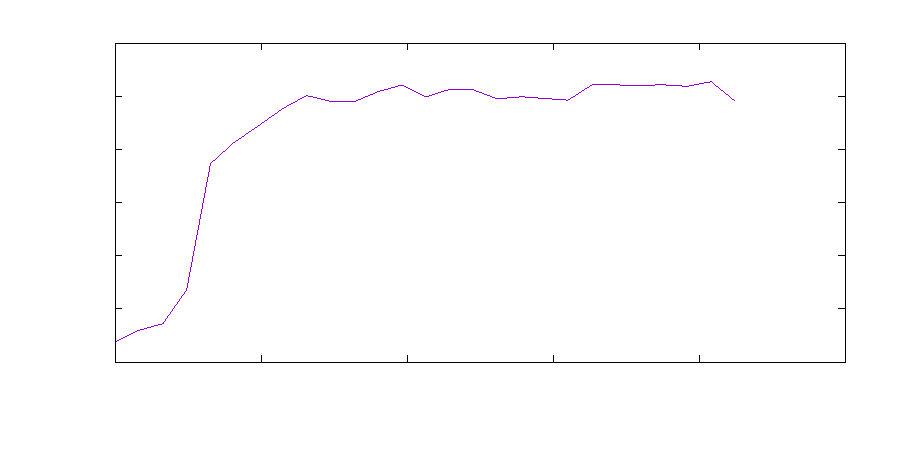
\includegraphics{../images/startup}}%
    \gplfronttext
  \end{picture}%
\endgroup

  \caption{Evolution of ozone after a long full stop of the
    generator.}
  \label{fig:long-stop}
\end{figure}
\begin{figure}[htbp]
  \centering
  % GNUPLOT: LaTeX picture with Postscript
\begingroup
  \makeatletter
  \providecommand\color[2][]{%
    \GenericError{(gnuplot) \space\space\space\@spaces}{%
      Package color not loaded in conjunction with
      terminal option `colourtext'%
    }{See the gnuplot documentation for explanation.%
    }{Either use 'blacktext' in gnuplot or load the package
      color.sty in LaTeX.}%
    \renewcommand\color[2][]{}%
  }%
  \providecommand\includegraphics[2][]{%
    \GenericError{(gnuplot) \space\space\space\@spaces}{%
      Package graphicx or graphics not loaded%
    }{See the gnuplot documentation for explanation.%
    }{The gnuplot epslatex terminal needs graphicx.sty or graphics.sty.}%
    \renewcommand\includegraphics[2][]{}%
  }%
  \providecommand\rotatebox[2]{#2}%
  \@ifundefined{ifGPcolor}{%
    \newif\ifGPcolor
    \GPcolorfalse
  }{}%
  \@ifundefined{ifGPblacktext}{%
    \newif\ifGPblacktext
    \GPblacktexttrue
  }{}%
  % define a \g@addto@macro without @ in the name:
  \let\gplgaddtomacro\g@addto@macro
  % define empty templates for all commands taking text:
  \gdef\gplbacktext{}%
  \gdef\gplfronttext{}%
  \makeatother
  \ifGPblacktext
    % no textcolor at all
    \def\colorrgb#1{}%
    \def\colorgray#1{}%
  \else
    % gray or color?
    \ifGPcolor
      \def\colorrgb#1{\color[rgb]{#1}}%
      \def\colorgray#1{\color[gray]{#1}}%
      \expandafter\def\csname LTw\endcsname{\color{white}}%
      \expandafter\def\csname LTb\endcsname{\color{black}}%
      \expandafter\def\csname LTa\endcsname{\color{black}}%
      \expandafter\def\csname LT0\endcsname{\color[rgb]{1,0,0}}%
      \expandafter\def\csname LT1\endcsname{\color[rgb]{0,1,0}}%
      \expandafter\def\csname LT2\endcsname{\color[rgb]{0,0,1}}%
      \expandafter\def\csname LT3\endcsname{\color[rgb]{1,0,1}}%
      \expandafter\def\csname LT4\endcsname{\color[rgb]{0,1,1}}%
      \expandafter\def\csname LT5\endcsname{\color[rgb]{1,1,0}}%
      \expandafter\def\csname LT6\endcsname{\color[rgb]{0,0,0}}%
      \expandafter\def\csname LT7\endcsname{\color[rgb]{1,0.3,0}}%
      \expandafter\def\csname LT8\endcsname{\color[rgb]{0.5,0.5,0.5}}%
    \else
      % gray
      \def\colorrgb#1{\color{black}}%
      \def\colorgray#1{\color[gray]{#1}}%
      \expandafter\def\csname LTw\endcsname{\color{white}}%
      \expandafter\def\csname LTb\endcsname{\color{black}}%
      \expandafter\def\csname LTa\endcsname{\color{black}}%
      \expandafter\def\csname LT0\endcsname{\color{black}}%
      \expandafter\def\csname LT1\endcsname{\color{black}}%
      \expandafter\def\csname LT2\endcsname{\color{black}}%
      \expandafter\def\csname LT3\endcsname{\color{black}}%
      \expandafter\def\csname LT4\endcsname{\color{black}}%
      \expandafter\def\csname LT5\endcsname{\color{black}}%
      \expandafter\def\csname LT6\endcsname{\color{black}}%
      \expandafter\def\csname LT7\endcsname{\color{black}}%
      \expandafter\def\csname LT8\endcsname{\color{black}}%
    \fi
  \fi
    \setlength{\unitlength}{0.0500bp}%
    \ifx\gptboxheight\undefined%
      \newlength{\gptboxheight}%
      \newlength{\gptboxwidth}%
      \newsavebox{\gptboxtext}%
    \fi%
    \setlength{\fboxrule}{0.5pt}%
    \setlength{\fboxsep}{1pt}%
\begin{picture}(4030.00,4030.00)%
    \gplgaddtomacro\gplbacktext{%
      \csname LTb\endcsname%
      \put(814,704){\makebox(0,0)[r]{\strut{}$80$}}%
      \put(814,1141){\makebox(0,0)[r]{\strut{}$100$}}%
      \put(814,1579){\makebox(0,0)[r]{\strut{}$120$}}%
      \put(814,2016){\makebox(0,0)[r]{\strut{}$140$}}%
      \put(814,2453){\makebox(0,0)[r]{\strut{}$160$}}%
      \put(814,2890){\makebox(0,0)[r]{\strut{}$180$}}%
      \put(814,3328){\makebox(0,0)[r]{\strut{}$200$}}%
      \put(814,3765){\makebox(0,0)[r]{\strut{}$220$}}%
      \put(946,484){\makebox(0,0){\strut{}$0$}}%
      \put(1483,484){\makebox(0,0){\strut{}$2$}}%
      \put(2021,484){\makebox(0,0){\strut{}$4$}}%
      \put(2558,484){\makebox(0,0){\strut{}$6$}}%
      \put(3096,484){\makebox(0,0){\strut{}$8$}}%
      \put(3633,484){\makebox(0,0){\strut{}$10$}}%
    }%
    \gplgaddtomacro\gplfronttext{%
      \csname LTb\endcsname%
      \put(176,2234){\rotatebox{-270}{\makebox(0,0){\strut{}Concentration [ppm]}}}%
      \put(2289,154){\makebox(0,0){\strut{}Time [min]}}%
      \csname LTb\endcsname%
      \put(2646,1537){\makebox(-200,0){\nfrac{} 1/2 h}}%
      \csname LTb\endcsname%
      \put(2646,1317){\makebox(-100,0){1 h}}%
      \csname LTb\endcsname%
      \put(2646,1097){\makebox(-100,0){2 h}}%
      \csname LTb\endcsname%
      \put(2646,877){\makebox(-100,0){4 h}}%
    }%
    \gplbacktext
    \put(0,0){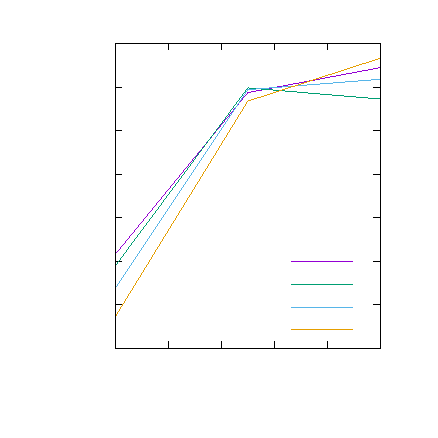
\includegraphics{../images/multi}}%
    \gplfronttext
  \end{picture}%
\endgroup

  \hfill
  % GNUPLOT: LaTeX picture with Postscript
\begingroup
  \makeatletter
  \providecommand\color[2][]{%
    \GenericError{(gnuplot) \space\space\space\@spaces}{%
      Package color not loaded in conjunction with
      terminal option `colourtext'%
    }{See the gnuplot documentation for explanation.%
    }{Either use 'blacktext' in gnuplot or load the package
      color.sty in LaTeX.}%
    \renewcommand\color[2][]{}%
  }%
  \providecommand\includegraphics[2][]{%
    \GenericError{(gnuplot) \space\space\space\@spaces}{%
      Package graphicx or graphics not loaded%
    }{See the gnuplot documentation for explanation.%
    }{The gnuplot epslatex terminal needs graphicx.sty or graphics.sty.}%
    \renewcommand\includegraphics[2][]{}%
  }%
  \providecommand\rotatebox[2]{#2}%
  \@ifundefined{ifGPcolor}{%
    \newif\ifGPcolor
    \GPcolorfalse
  }{}%
  \@ifundefined{ifGPblacktext}{%
    \newif\ifGPblacktext
    \GPblacktexttrue
  }{}%
  % define a \g@addto@macro without @ in the name:
  \let\gplgaddtomacro\g@addto@macro
  % define empty templates for all commands taking text:
  \gdef\gplbacktext{}%
  \gdef\gplfronttext{}%
  \makeatother
  \ifGPblacktext
    % no textcolor at all
    \def\colorrgb#1{}%
    \def\colorgray#1{}%
  \else
    % gray or color?
    \ifGPcolor
      \def\colorrgb#1{\color[rgb]{#1}}%
      \def\colorgray#1{\color[gray]{#1}}%
      \expandafter\def\csname LTw\endcsname{\color{white}}%
      \expandafter\def\csname LTb\endcsname{\color{black}}%
      \expandafter\def\csname LTa\endcsname{\color{black}}%
      \expandafter\def\csname LT0\endcsname{\color[rgb]{1,0,0}}%
      \expandafter\def\csname LT1\endcsname{\color[rgb]{0,1,0}}%
      \expandafter\def\csname LT2\endcsname{\color[rgb]{0,0,1}}%
      \expandafter\def\csname LT3\endcsname{\color[rgb]{1,0,1}}%
      \expandafter\def\csname LT4\endcsname{\color[rgb]{0,1,1}}%
      \expandafter\def\csname LT5\endcsname{\color[rgb]{1,1,0}}%
      \expandafter\def\csname LT6\endcsname{\color[rgb]{0,0,0}}%
      \expandafter\def\csname LT7\endcsname{\color[rgb]{1,0.3,0}}%
      \expandafter\def\csname LT8\endcsname{\color[rgb]{0.5,0.5,0.5}}%
    \else
      % gray
      \def\colorrgb#1{\color{black}}%
      \def\colorgray#1{\color[gray]{#1}}%
      \expandafter\def\csname LTw\endcsname{\color{white}}%
      \expandafter\def\csname LTb\endcsname{\color{black}}%
      \expandafter\def\csname LTa\endcsname{\color{black}}%
      \expandafter\def\csname LT0\endcsname{\color{black}}%
      \expandafter\def\csname LT1\endcsname{\color{black}}%
      \expandafter\def\csname LT2\endcsname{\color{black}}%
      \expandafter\def\csname LT3\endcsname{\color{black}}%
      \expandafter\def\csname LT4\endcsname{\color{black}}%
      \expandafter\def\csname LT5\endcsname{\color{black}}%
      \expandafter\def\csname LT6\endcsname{\color{black}}%
      \expandafter\def\csname LT7\endcsname{\color{black}}%
      \expandafter\def\csname LT8\endcsname{\color{black}}%
    \fi
  \fi
    \setlength{\unitlength}{0.0500bp}%
    \ifx\gptboxheight\undefined%
      \newlength{\gptboxheight}%
      \newlength{\gptboxwidth}%
      \newsavebox{\gptboxtext}%
    \fi%
    \setlength{\fboxrule}{0.5pt}%
    \setlength{\fboxsep}{1pt}%
\begin{picture}(4030.00,4030.00)%
    \gplgaddtomacro\gplbacktext{%
      \csname LTb\endcsname%
      \put(814,704){\makebox(0,0)[r]{\strut{}$200$}}%
      \put(814,1010){\makebox(0,0)[r]{\strut{}$220$}}%
      \put(814,1316){\makebox(0,0)[r]{\strut{}$240$}}%
      \put(814,1622){\makebox(0,0)[r]{\strut{}$260$}}%
      \put(814,1928){\makebox(0,0)[r]{\strut{}$280$}}%
      \put(814,2235){\makebox(0,0)[r]{\strut{}$300$}}%
      \put(814,2541){\makebox(0,0)[r]{\strut{}$320$}}%
      \put(814,2847){\makebox(0,0)[r]{\strut{}$340$}}%
      \put(814,3153){\makebox(0,0)[r]{\strut{}$360$}}%
      \put(814,3459){\makebox(0,0)[r]{\strut{}$380$}}%
      \put(814,3765){\makebox(0,0)[r]{\strut{}$400$}}%
      \put(946,484){\makebox(0,0){\strut{}$0$}}%
      \put(1245,484){\makebox(0,0){\strut{}$5$}}%
      \put(1543,484){\makebox(0,0){\strut{}$10$}}%
      \put(1842,484){\makebox(0,0){\strut{}$15$}}%
      \put(2140,484){\makebox(0,0){\strut{}$20$}}%
      \put(2439,484){\makebox(0,0){\strut{}$25$}}%
      \put(2737,484){\makebox(0,0){\strut{}$30$}}%
      \put(3036,484){\makebox(0,0){\strut{}$35$}}%
      \put(3334,484){\makebox(0,0){\strut{}$40$}}%
      \put(3633,484){\makebox(0,0){\strut{}$45$}}%
    }%
    \gplgaddtomacro\gplfronttext{%
      \csname LTb\endcsname%
      \put(176,2234){\rotatebox{-270}{\makebox(0,0){\strut{}Concentration [ppm]}}}%
      \put(2289,154){\makebox(0,0){\strut{}Time [min]}}%
    }%
    \gplbacktext
    \put(0,0){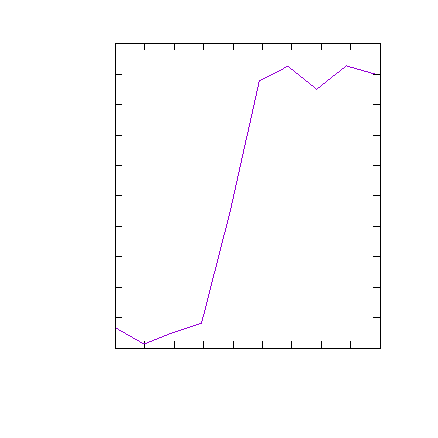
\includegraphics{../images/current}}%
    \gplfronttext
  \end{picture}%
\endgroup

  \caption{Left: Evolution of the ozone concentration after a full stop of the
    generator for different waiting times. Right: ozone level
    dependence on current of Mercury lamp. The steep
    flank occured after a change of the current from
    \SI{10}{\milli\ampere} to \SI{17}{\milli\ampere}.}
  \label{fig:multiple-stop}
\end{figure}

After determining the longtime behaviour, I was interested in
short term pauses. For that reason I stopped the generator (after it
had stabilized) for {\nfrac{} 1/2} \si{hour}, \SI{1}{\hour},
\SI{2}{\hour} and \SI{4}{\hour} and measured the startup time. The
result can be found in Figure~\ref{fig:multiple-stop}
lefthandside. Since the time resolution of the DOAS instrument is
rather coarse the only safe statement is, that even after a
\SI{4}{\hour} stop the concentration climbed back up to around
\SI{200}{ppb} after \SI{5}{\minute}. So it stands to reason, that if
the device is used regularly a prolonged startup time should not be an
issue, even if one sticks to the constant flow of $\Phi_{\ch{O3}} =
\SI{0.03}{\liter\per\minute}$.

As compared to the ozone level in Figure~\ref{fig:long-stop}, the
plateau seems to lie slightly lower in this second experiment. The
reason for this lies most probably in the stabilization of the Mercury
lamp, which was factory new during the first measurements.

After having analyzed the startup procedure, I wanted to investigate
the qualitative influence of the power supply current of the Mercury
lamp on the ozone concentration. Beforehand it was not clear whether a
higher current would increase or decrease the ozone production rate,
as, as was described in Section~\ref{sec:theory-ozone}, I did not know
how a change in power would transform the power distribution on the
different Mercury lines. I recorded a time series while switching
between the two possible currents, \SI{10}{\milli\ampere} and
\SI{17}{\milli\ampere}, and yielded Figure~\ref{fig:multiple-stop}
righthandside. From this one can see that generator still works in a
regime where a higher current leads to more ozone. However, this fact
is secondary in nature for my purposes, as I do not wish to maximize
the ozone output. \SI{200}{ppm} ozone allows for the minimization of
the ozone generator flow entering the sample air stream, minimizing
the effects due to dillution, while still supplying enough ozone for
the conversion. Thus any ozone concentration in this region is well
suited for my purposes, hence I always applied the preset current to
the Mercury lamp.

%%% Local Variables: 
%%% mode: latex
%%% TeX-master: "../Bachelor"
%%% End: 

\cleardoubleoddstandardpage{}

\printbibliography[heading=bibintoc]

%%% Local Variables: 
%%% mode: latex
%%% TeX-master: "Bachelor"
%%% End: 




\cleardoubleoddstandardpage{}
\selectlanguage{german}
  
\subsubsection*{Erklärung}
\label{sub:Erklärung}

Ich versichere, dass ich diese Arbeit selbstständig verfasst und keine 
anderen als die angegebenen Quellen und Hilfsmittel verwendet habe.

\vspace{2\baselineskip}

Heidelberg, den 25.\ April 2016 \hspace{5em} \hrulefill

\selectlanguage{english}

%%% Local Variables: 
%%% mode: latex
%%% TeX-master: "../Bachelor"
%%% End: 


\end{document}

%%% Local Variables: 
%%% mode: latex
%%% TeX-master: t
%%% End: 
